\documentclass[]{article}
\setlength{\parskip=0.7}{\baselineskip}
\setlength{\parindent}{0pt}

\usepackage{times}
\usepackage{fullpage}

\usepackage{epsfig}
\usepackage{subfigure}

\usepackage{listings}
\usepackage{siunitx}
\usepackage[super]{nth}

\usepackage[sharp]{easylist}

\usepackage[table,xcdraw]{xcolor}

\usepackage{algorithm}
\usepackage{algpseudocode}
\algblockdefx[Struct]{Struct}{EndStruct}%
  [1]{Begin Journal Entry: #1 }%
  {End Entry}

\definecolor{NavyBlue}{cmyk}{0.94,0.54,0,0.5}
\definecolor{BrickRed}{cmyk}{0.16,0.89,0.61,0.2}
\usepackage{url}
\usepackage{breakurl}

\usepackage[
        colorlinks=true,
        urlcolor=NavyBlue, 
        linkcolor=NavyBlue, 
        bookmarksopen=true]{hyperref}
\hypersetup{
    colorlinks,citecolor=NavyBlue,
    linkcolor={red!50!black},
    urlcolor={blue!90!black}
}


\newcommand{\us}{$\mu$s }
\newcommand{\subtopic}[1]{\vspace{1.5pt} \noindent \textbf{#1}}

\definecolor{notecolor}{rgb}{0.75,0,0} % A darker red
\definecolor{hlcolor}{RGB}{0,0,205}
\newcommand{\todo}[1]{\textcolor{notecolor}{\textbf{TODO: #1}}}
\newcommand{\hl}[1]{\textcolor{hlcolor}{#1}}
\newcommand{\fixit}[2][]{\textcolor{notecolor}{%
     \ifthenelse{\isempty{#1}}{\textbf{[Fixit: %
         #2]}}{\textbf{#2\footnote{\textcolor{notecolor}{Fixit: #1}}}}}}
\newenvironment{highlight}{\par\color{notecolor}}{\par}





\begin{document}

\title{Kawkab: A Distributed Filesystem for Fast Data}
%\author{Sajjad Rizvi, Bernard Wong}
\date{}
\maketitle

\bgroup
\def\arraystretch{1.5}
\begin{table}[!htb]
\centering
\caption{Change Log}
\label{table:change-log}
\begin{tabular}{|l|l|l|}
\hline
\rowcolor[HTML]{EFEFEF} 
Date             & Description  & Participants  \\ \hline
 March 20, 2018  & Restructured the docuemtn and added the section ``Current Distributed Design'' & Sajjad \\ \hline
 March 03, 2017  & Kawkab single node design           & Sajjad  \\ \hline
 March 10, 2017  & - Added sections 3 and 4, about the distributed design of Kawkab& \\ 
                 & - Updated architecture diagram & Sajjad  \\ \hline
 August 11, 2017  & Kawkab single node design updated  & Sajjad  \\ \hline
\end{tabular}
\end{table}
\egroup


\section{Introduction} 

Kawkab is a distributed filsesystem developed to efficiently manage large
amounts of streaming data. Unlike traditional filesystem that are designed for
bulk data transfers in the context of Big Data, Kawkab manages the storage of
fast streaming data with the primary focus on memory management, read and write
performance, and scalability.


Kawkab's design is mainly motivated from the design approach of a standard Unix
filesystem.  However, unlike a disk-based traditional filesystem, Kawkab is an
append only system,  and the location of the blocks is not fixed to a specific
storage medium. Kawkab assumes the availability of an extensible backend or
\textit{global storage} that can store large volumes of data. Unlike other
distributed filesystems such as Tachyon, Kawkab allows to read most recent data
of the files even if the last block of the file is not completely filled with
the file's data. 
%The reasons to follow the Unix filesystem is to control the memory usage of
%the system and make the system memory efficient.

Kawkab is designed for the single writer and multiple readers use case. Kawkab
allows only one node at a time to perform file append operations. Moreover,
the file appender is restricted to be a distinguished node that created
the file. Other nodes can only read the files.


This document describes the architecture and design of Kawkab. 

\section{Workload}

Kawkab is specifically designed for fast streaming data workload, which is
common in financial industry.  The workload may consist of unstructured blobs
or structured records.  Kawkab supports data writing only at the end of the
file, i.e., Kawkab is an append-only filesystem. The readers are allowed to
read from any file location, including the most recent data written in the
file.  However, the most recent data can be read with some bounded staleness.
The workload may consist of any ratio of read and write requests.  Readers are
allowed to read data from any node in the system. However, a file writer can
only writer through a specific node in Kawkab.  The clients can concurrently
read and write large volumes of files. However, only one writer is allowed per
file at a time. Multiple readers and the writer can concurrently read and write
the file at the same time.

%Todo: Data access frequency and size, number of readers per node, number of
%nodes where readers are located $\ldots$.




\section{Architecture} 

%\begin{figure}[t]
%    \centering
%    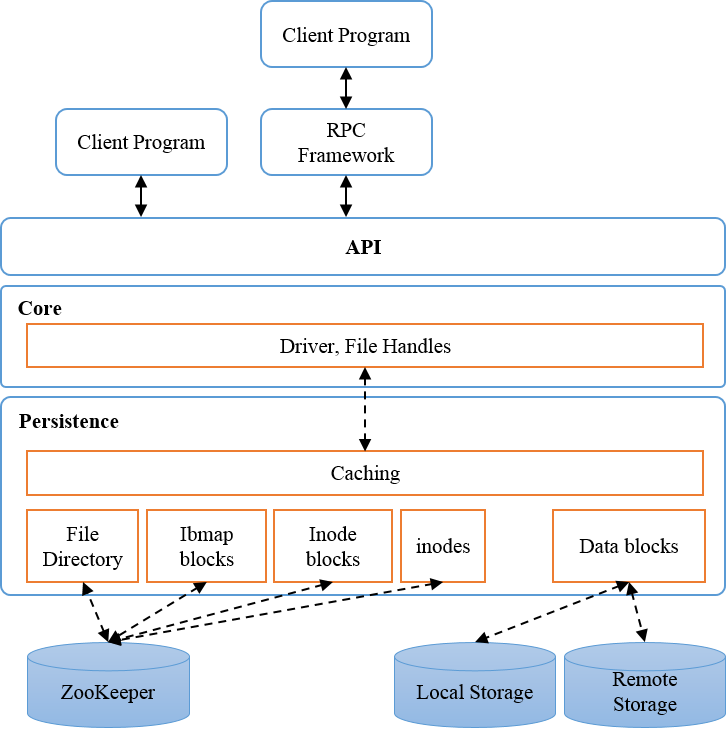
\includegraphics[width=0.7\columnwidth]{{figures/architecture.png}}
%    \caption{Kawkab architecture}
%   \label{fig:architecture}
%\end{figure}


\begin{figure}[t]
    \centering
    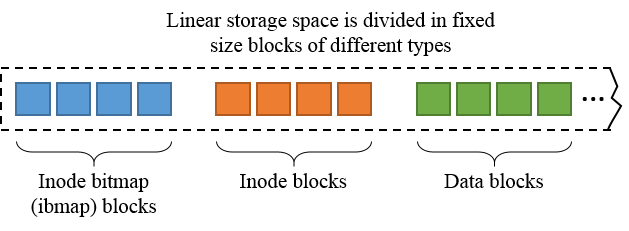
\includegraphics[width=0.5\columnwidth]{{figures/linear-space.png}}
    \caption{Filesystem is designed as a very large storage space organized in fixed size blocks}
   \label{fig:storage-space}
\end{figure}

\begin{figure}[t]
    \centering
    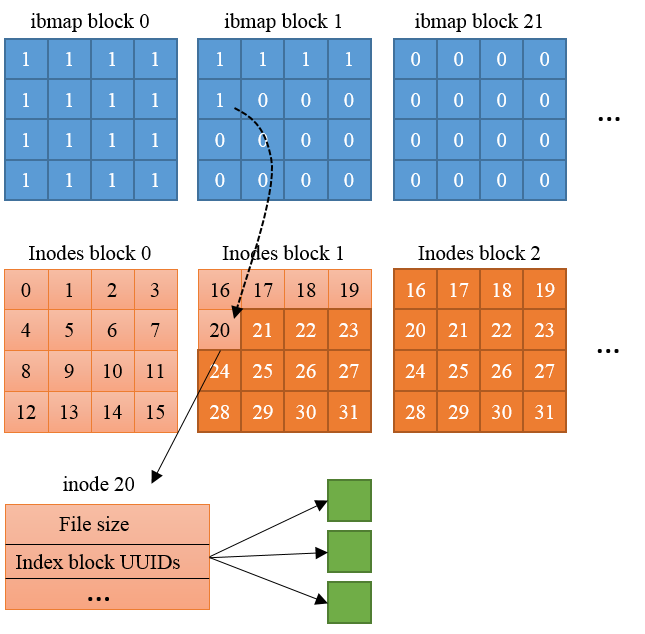
\includegraphics[width=0.4\columnwidth]{{figures/blocks-layout.png}}
    \caption{Relationship between different types of blocks}
   \label{fig:blocks-layout}
\end{figure}


\begin{figure}[t]
    \centering
    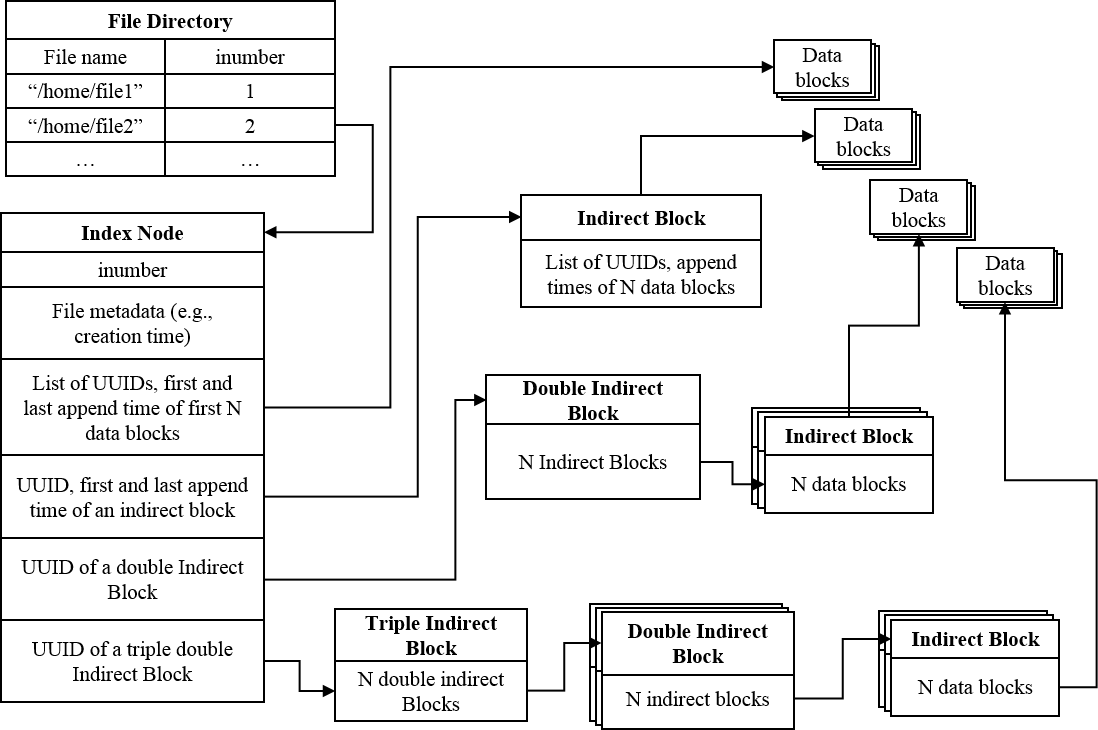
\includegraphics[width=0.5\columnwidth]{{figures/file-index-design.png}}
    \caption{File directory and file index}
   \label{fig:data-structures}
\end{figure}




At the high level, the system consists of four fixed size structures: a file directory,
inode-bitmap blocks, inode blocks, and data blocks.


\subsection{Namespace and File Directory}
A file consists of metadata and fixed size data blocks that are persistently
stored in an extensible storage such as Amazon S3 or Dynamo.
Each file has a unique fully qualified name, which a client assigns when the client
creates the file. The clients access the files using the filenames.
However, internally, Kawkab assigns a globally unique 64-bit number to each file, which is
called \textit{inumber}. Internally the files are referred through 
their inumbers. The filename to inumber mappings are stored in the \textit{file directory},
which is explained in the next section.

Kawkab does not support directory hierarchies. Instead, all the files are stored
as a flat storage system. However, the filenames can be qualified to represent
directories, e.g., ``/home/smash/file''.

\subtopic{File Directory:}
In our current design, the file directory is implemented as a distributed
key-value store, where the keys are the filenames and the values are the corresponding
inumbers. We propose to use ZooKeeper as the key-value store because of its
atomic \textit{znode}-creation functionality that returns an error if
the \textit{znode} already exists. However, any distributed key-value store can be used 
that provides atomic updates to the key-value store.


\subsection{Inode Bitmap Blocks}
A node keeps track of the assigned and available inumbers using an \textit{inodes-bitmap}.
Each node has a fixed size inodes-bitmap, which is divided in several sequential blocks
called \textit{ibmap-blocks}. Each bit in the bitmap translates to an index in the
\textit{inodes-block} structure, which is further explained below.
Figure~\ref{fig:blocks-layout} shows the relationship between the ibamap blocks, 
inode blocks, and the data blocks. Each bit at index $i$ in the
ibmap indicates whether inumber $i$ or the inode at index $i$ in the inodes-blocks
is already used or not.

\subtopic{Inumber Assignment:}
A node linearly searches the ibmap-blocks to find the next unset bit in the ibmap.
To optimize the search, the node starts searching from the last position it
found the unused bit. When a file is deleted, which we expect to be extremely
rare, the bit is unset in the ibmap.


%An inode bitmap block, or ibmap block, is a
%fixed size block that contains part of the ibmap.  
%When a new file is created, Kawkab scans the ibmap to find the first unused 
%inumber and assigns that inumber to the inode associated with the file. Moreover,
%Kawkab sets the bit in the bitmap that is associated with the inumber.
%When a file is deleted, Kawkab clears the bit in the ibmap, which allows
%Kawkab to reuse the inode and the inumber for the next new file.

\subtopic{Metadata Partitioning:} As the system consists of several nodes,
different nodes can concurrently create files that lead to inumber conflicts,
i.e., different nodes assigning same inumber to different files.  In order to
avoid inumber conflicts and to  consistently maintain metadata without
significant communication overhead between the nodes, the 64-bit space of
inumbers is linearly partitioned across the nodes. A node assigns a unique
inumber to a new file only from its own partition. This ensures that a node can
assign an inumber to a file without communicating over the network and without
consensus with the other nodes.

Partitioning splits the 64-bit inumber space across all the nodes that may lead to
two problems. First, a node may run out of the inumbers in its partition, which
will prevent the node from creating new files.  However, this is highly
unlikely due to the large size of partition assigned to each node. For example, if
the system is designed for $2^{20}$ nodes (1.04 million nodes), each nodes is
assigned nearly $2^{63} / 2^{20} = 2^{43} = 8.79 * 10^{12}$ inumbers, which is a
sufficiently large partition for a single node. If a node creates a new file
every 100 microseconds, i.e., $10000$ files per second, it will take almost
$39.7$ years to run out of the inumbers. In addition to the large partition
sizes, a node reuses a file's inumber when the file is deleted.

The second problem is about running out of inumber-partitions, which will
prevent adding more nodes in the system. For example, if the nodes fail and the
new nodes join enough number of times that exceed the maximum number of nodes
(1.04 million in the previous example), the system can run out of inumbers
globally. To prevent this situation, Kawkab allows reassigning partitions to
other nodes. A new node can be assigned the partition of the previously failed
node.

%To prevent a node from running out of inumbers,
%the inumbers of the deleted files are reused.  Moreover, a failed node's shard
%can be reassigned to another node in order to prevent the filesystem from
%running out of the inumbers.  

\subtopic{Storing Partitions' Information:} The inumber partitioning
information is stored in a distributed key-value store such as ZooKeeper, where
the keys are the node IDs and the values are the inumber-ranges assigned to the
nodes.  A distributed KV store does not become the performance bottleneck in
this case because the nodes' churn rate is very low.  The system ensures that
the inumber-ranges assigned to different nodes are disjoint. [This functinlaity
is not implemented yet. Currently the partitioning is static in which a 
predifined size partition is assigned to a node based on its node ID.]


%[TBD: How to ensure that the ranges are non-overlapping?]


%A virtual file comprises of metadata and data blocks.  The storage space is a
%collection of fixed size blocks $\{B_1, B_2, \ldots, B_N\}$.  Each block has a
%unique ID (UUID), and the blocks are persistently stored as files on the local
%storage devices (HDDs, SSDs) and the cloud, e.g., Amazon S3.
%
%The blocks in the storage space are of three types: index-node-bitmap blocks,
%index-node blocks, and data blocks.

\subsection{Inodes and Inodes-blocks} 

Each node is assigned a predefined number of \textit{index-node blocks}
(\textit{inodes blocks}) where an inodes-block is a fixed size structure
consisting of a number of \textit{index-nodes} (\textit{inodes}).  An inode
is the main structure that keeps track of the file metadata that associates
data blocks with the files.


\subtopic{Inode:} Kawkab stores metadata of a file in a fixed size structure
called \textit{index node} or \textit{inode}. An inode is uniquely identified by
the \textit{inumber} assigned to the file with which the inode is associated.

An inode contains metadata information that includes the current file size 
and other information such as file creation time. In addition, an inode includes
the IDs of the blocks that store the data-index of the file.
\hl{TBD: More about index storage when we add time series index in the
filesystem.}


%\hl{TODO: Update the following list to mention that the indirect blocks
%only contains the indices for the data, not the actual data blocks.
%The data blocks are identified and accessed using their IDs which
%is a combination of inumber and the block number.}
%
%\begin{enumerate}
%  \item \subtopic{File Metadata:} The file metadata consists of information
%        about the file such as file creation time, last access time, file
%        rights, and file size.
%
%	\item \subtopic{First $N$ Data Index Blocks:} An inode contains a fixed number
%$N$ of the IDs of the first $N$ data index blocks associated with the file.
%A data index block contains the indices of the data stored in the data blocks
%associated with the file.
%The number $N$ is kept small to optimize for the memory space and the file
%access for smaller files. 
%
%  \item \subtopic{Indirect Block:} 
%An inode contains the ID of one indirect block, where an indirect block is
%special data block that only consists of the IDs of the data blocks associated
%with the file. Thus, an indirect block is level-1 index into the file.
%As the size of each block is fixed, an indirect block contains the
%IDs of a fixed number of data blocks in a file. These data blocks 
%range from $N+1$ to $M$ where $M$ is the number of IDs stored in the
%direct block.
%
%  \item \subtopic{Double and Triple Indirect Block:}
%An inode has one double and one triple indirect block. A double indirect block is a two
%level index, i.e., a double indirect block is the ID of a special data block that contains
%the IDs of indirect blocks. Similarly, a triple indirect block contains the IDs of the
%double indirect blocks. These indexing levels are sufficient to support the maximum 
%file size in Kawkab, which is $2^{63}-1$ bytes.
%
%\end{enumerate}

\subtopic{Inode Blocks:} A collection of inodes are stored in a fixed size
structure called \textit{inode block}. An inode block consists of a fixed
number of a continuous series of inodes. 


\subtopic{Locating an inodes-block:} An inodes-block is uniquely identified by
the inodes-block number.  Because the inodes-blocks are fixed size and contains a
fixed number of inodes, the block number can be easily calculated from the
\textit{inumber} assigned to the file.
%, which is briefly described as follows.  As each inode has a fixed size $S_I$
%bytes, an inode block $B$ contains $N = S_{B} / S_I$ number of inodes, where
%$S_B$ is the size of an inodes block.  Thus, the inumber $x$ is located in the
%inode block number $ x / N$. In this way, given an inumber, Kawkab can
%calculate number of the inode block that contains the associated inode, and
%the index of the inode inside the block.
Figure~\ref{fig:blocks-layout} depicts the way in which ibmaps, inode blocks, and
inodes are related to each other.

%When a file is created, the file is assigned a unique inumber, which is the
%first available inode number in the system. To achieve that, the system keeps
%track of the inumbers already assigned using a bitmap called \textit{inode
%bitmap} or \textit{ibmap}. The ibmap is stored in the blocks of type "inode
%bitmap block".

%\subsection{Data Blocks} Kawkab has fixed size data blocks. Each data block has
%a unique ID, generated as a UUID.  Each block is persistently stored as a file
%in the persistent storage of the system, e.g., local or remote disks, EB3, or
%S3.  The name of the persistent file is extracted from the UUID: the UUID is
%converted to an ASCII character string using Base64 encoding.  The ASCII name
%is then converted into a file path such that each two characters in the ASCII
%representation of the UUID become a directory name in the persistent storage.
%For example, a UUID \texttt{ABCDEFGH} is stored as a file
%\texttt{/storage/datablocks/AB/CD/EF/GH}.


\subsection{Data blocks}

Data blocks contain the actual data belonging to the files in the system.
Each file is divided into fixed-size blocks that are stored persistently in
the global storage. Initially a block is created and filled with data
in the local storage. When the block becomes full, it is sealed and transferred 
to the global storage. Data blocks are immutable once they are transferred
to the global storage. However, this can restrict transferring incomplete
blocks to the global storage that may prevent creating new blocks locally.
This problem is solved through multi-version blocks, which we discuss
further later in this document.

All of the files in the filesystem have same and fixed size of data blocks. 
Kawkab stores individual data blocks as actual files in the underlying 
local storage and the global storage. Therefore, it is recommended that 
a larger block size is used for local and global 
storage efficiency. 

\subtopic{Segments in Blocks:} Each data block is further partitioned into
fixed size segments for better memory management. For example, a 64MB data
block can be partitioned into 64 segments of size 1MB.  
%A block is not physically partitioned as segments on the local or global
%storage. Instead, a segment is just an abstraction for better memory
%management. 
The blocks are loaded into memory in segments instead of blocks, which reduces internal
fragmentation in memory.  During the file read and append operations, the cache
sub-system of Kawkab reserves memory for a segment instead of a block. As a
result, a large number of partially filled blocks do not waste a large portion
of memory. For instance, if 1000 files are concurrently being appended, the
cache requires 1000 1MB-segments in memory instead of 1000 64MB-blocks.


%The readers read the blocks from the global storage if the block is
%not in both its cache and its local storage. The file read operation is further
%explained in the section~\ref{}. 

\subtopic{Records in Segments:} 
Kawkab supports two types of files: binary files and structured files.
Each type has different way of reading from and appending data to the files.
For the binary files, data is read and appended using a blob of bytes.
Structured files are read and appended using fixed-size structures
called \textit{records}. A record is a user-defined structure that
the user provides during the file creation process.
For simplicity and correctness, Kawkab does not allow mixing the file
types,
%~\footnote{Todo: We need to detect the type of record in each operation. We
%should not allow mixed record structure in a file.}
i.e., mixing binary and
structured files and mixing different record structures for the same file.
%Kawkab supports two types of file append and
%read operations. Files can be appended using a given blob of bytes or using
%user defined fixed-size structures called \textit{records}. 

%Reads and appends using an array of bytes can be viewed as an array of one-byte
%records. Thus, 

In a structured file, a data segment consists of several records, which may not
align with the segment boundary. For example, 76 bytes are left if 100-byte
records are stored in a segment of 1MB. For simplicity, Kawkab does not store
records across segments.  Instead, Kawkab uses padding to fill a segment and
does not distribute records across multiple segments. To achieve this, Kawkab
imposes the restriction that the record sizes must be smaller or equal to the
segment size in the system. 


%To associate the blocks with a file, the
%blocks are indexed using a structure called \textit{index node} or

\subtopic{Block and Segment IDs:} Each data block is uniquely identified with
the inumber and the block index in the file.  The block index is calculated
from the byte offset in file.  A segment ID is a combination of the inumber of
the file, the block index in the file, and the segment index in the block.


\subtopic{Locating File Segments and Blocks:} Locally the blocks are stored as
individual files.  Kawkab converts a block ID to a Base64 encoded string. The
encoded string then represents the file path in the local storage as well as
the file path or the key in the global storage.

The Base64 encoded string is converted to a path in the following way.  The
string is divided in words of size 3. The first six words denote the
directories. The rest of the letters in the string denote the file name in the
last directory. To avoid weird file names, we use the modified version of
Base64 encoding that only uses the readable characters in the encoded string.




\subsection{File Access Patterns}

\subtopic{File Writes:} Kawkab allows only one writer at a time to write the
file. The first client that opens the file becomes the distinguished writer of
the file until the writer closes the file. Only the distinguished writer is
then allowed to append to the file. Moreover, the node where the client is
located becomes the \textit{primary node} of the file.  The other nodes may
fetch recent appends from the primary node when the data is not replicated in
the global storage.

If an existing writer fails, another client can become the distinguished writer
by successfully opening the file for writing. If the writer closes the file,
another writer can open the file and become the distinguished
writer\footnote{In the Smash's use case, files are never closed.}. However,
Kawkab allows only one file writer at a time.

Each append request consists of small number of bytes, e.g., less than 100 bytes.

\subtopic{File Reads:}
Kawkab allows multiple readers to read at the same time. If the data block
is not located locally in the system, the data block is fetched from the global storage if
it is available. If the data block is not available in the global storage, the data block
is fetched from the node where the file-writer is located.





\section{Memory and Storage Management}

Kawkab divides storage in three categories: main memory, local storage, and global
storage. These categories are used in hierarchy. Initially all the data
is created or updated in memory. The main memory data is synchronized to the
local storage temporarily. Eventually, all the data is moved to an extensible
and permanent global storage.


\subsection{Main Memory}

Each node is assigned a fixed size of RAM, which the node uses 
for all the objects including file segments, ibmaps, inode blocks, and
file directory. The main memory is divided into two parts: (1) a large
unified cache for data segments, ibmaps, and inodes blocks, and (2) a small
buffer to read blocks from other nodes.
%, and (3) another small buffer for the file directory.


\subtopic{(1) LRU Cache:} 

A large portion of the memory is used as a unified LRU cache for data segments,
ibmaps, and inodes-blocks.  A file's read and append operations require access
to an inodes-block as well as a data block. Moreover, a file's creation and
deletion operations additionally require access to the file directory and the
ibmap blocks. If the accessed blocks are not already in the cache, the cache
loads the required blocks into the cache.  If the cache does not have free
memory space to load a required block or segment, it evicts an existing block
from the memory to create the space for the incoming block. 

\subtopic{Eviction Policy:} Currently the blocks are evicted based on the LRU
policy.  If the LRU block is dirty, which is unlikely to happen in the normal
scenarios, the evicted block is first flushed to the local storage and then
evicted. Otherwise, the non-dirty LRU block is simply deleted from the memory.
Flushing the dirty block during eviction  slows down the file operation that
caused eviction, which automatically adds back pressure to reduce workload on
the node.


%\subtopic{(2) Remote Blocks Buffer:}
%
%A remote-blocks buffer is a relatively a small
%portion of memory that is reserved to read recently updated blocks from
%other nodes.  If a data block is not yet stored in the global storage, a node
%can optionally read the block from the file's primary node, where the file
%writer is located, that always has the most recent file data. These blocks 
%that are read from the remote nodes are stored in the remote-blocks buffer.  
%The blocks are deleted from the buffer at the end of the read operation.
%
%- TOOD: Whey we have not merged this buffer with the main Cache?
%


%\subtopic{(3) File Directory Buffer:} 
%
%The file directory buffer stores a portion of
%the file directory in memory.  A part of the file directory is kept in memory
%to speed up the file open operations that require the file's inumber.  When a
%node receives a file open request, it checks in the buffer whether it has the
%filename to the inumber mapping in its local cache. If the node does not have
%the mapping, it fetches the mapping from the global file directory and caches
%the information. In this way, the first open request may be slow. However, the
%subsequent file open requests are fast.
%
%Note that the file directory is only accessed during the file open/create and
%file delete operations.
%
%\subtopic{Eviction Policy:} We use LRU based eviction policy for the
%file directory buffer.
%

\subsection{Local Storage} Each node contains one or more SSDs that are used as
a temporary local storage for ibmaps, inode blocks, and data blocks.  The local
storage is used as a temporary staging area for the new data blocks and the
modified ibmaps and inodes-blocks.  The main purpose of the local storage is
(1) to provide fault tolerance to some extent, and (2) to provide a temporary 
large storage in order to keep up with the peak data ingestion rates.

During the file append operations, the appended segments in memory are flushed
to the corresponding blocks on the local storage.  The data blocks that become
full (i.e., all of their segments are filled with the file data)
are transferred to the global storage.  Other blocks, such as ibmaps and
inode blocks, are periodically synced to the global storage.

Like the main memory cache, local storage is also managed as an evictable
staging area. The blocks that are synced to the global/persistent storage are
marked as deletable. When the local storage is full up to a threshold, Kawkab
deletes the globally synced blocks to keep the storage usage up to
the defined threshold.

In the local storage, the blocks are saved as individual files. The actual
file location in the local storage is based on the block ID.

%- TODO: Blocks eviction policy: a complicated LRU policy that is based on the
%  access pattern of the main memory cache. It also needs a probabilistic
%  data structure that encodes the IDs of all the locally stored blocks.
%
%- TODO: Impact of small file sizes: slows down performance.
%
%- TODO: Impact of a large number of files in one directory in the underlying storage
%
%- TODO: What if the local storage is full?
%

\subsection{Global storage}

The global storage persistently stores all the blocks. Any extensible storage
technology can be used as the global storage, e.g., Amazon S3, Dynamo, HDFS, a
distributed key-value store, etc. However, the major requirement is that the 
global storage is scalable and directly accessible to all the nodes in the system.

Ibmaps and inode blocks are not append-only blocks. Therefore, their
synchronization with the global storage is different than the data blocks,
which are append-only blocks. Ibmaps and inodes-blocks are frequently updated
during different file operations. Ibmap modifications are less frequent than
the inodes-blocks modifications. An ibmap is only modified when a new file is
created or an existing file is deleted.  However, an inodes-block is modified
after each append operation because the file size is updated in
the inode after each append operation. Therefore, ibmaps and inodes blocks are
periodically flushed to the local storage for fault tolerance.  Moreover, these
blocks are periodically updated in the global storage as well for persistence
and availability to the other nodes.


\subtopic{Global Store Assumptions:}

We assume the following properties for the global store:

\begin{itemize}

\item Highly available: The global store is always available to at least all
  of the file writers.

\item Globally accessible: Data store is concurrently accessible by all of the nodes
  in the Kawkab cluster.

\item Highly scalable: The throughput of the global store remains up to an
acceptable threshold with the increase in the number of nodes in the Kawkab cluster.

\end{itemize}


%\begin{figure}[t]
%    \centering
%    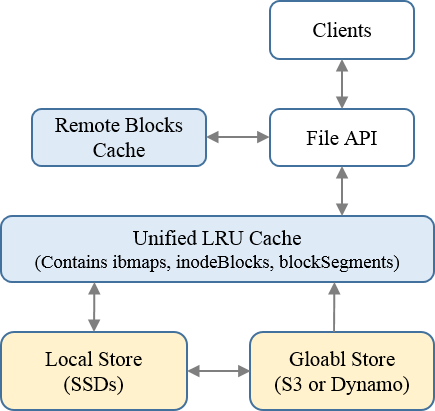
\includegraphics[width=0.4\columnwidth]{{figures/block-diagram.png}}
%    \caption{[TBD: caption] Block diagram.}
%   \label{fig:block-diagram}
%\end{figure}



%\subsection{File Directory} Kawkab filesystem contains a file directory that
%defines the namespace of the system.
%%The file directory keeps track of the existing files in the system and the way
%%to access the files.
%Each file in the system has a unique name and a unique inode number.  The file
%directory is a simple collection of $\langle$ file name, inode number $\rangle$
%pairs that maps a file name to an inode number.  The clients refer to a file
%using the file name whereas the system access the files through the inode
%numbers. 
%
%The file directory is the only structure that keeps the mapping of the file
%names and the inode numbers. Therefore, the file directory is made persistent
%and consistent through a distributed key-value store such as ZooKeeper.
%
%\subtopic{File Namespace:} Kawkab has a flat namespace. Kawkab does not maintain
%directory hierarchies. However, a user can use any file name.
%
%



\section{File Operations}

Kawkab supports the following file operations:

\subsection{File Open}

A client opens a file to read or to append the file. If the file is opened for
appending, the file is first created if it does not already exist.

\subtopic{File Creation:} File creation is an atomic operation, which is
performed as follows.
%The node first acquires the file-specific lock that prevents multiple clients
%from creating the same files at the same time.  
The node first assigns an unused inumber from its inumber-partition to the new
file.  The node then atomically adds a new filename-to-inode mapping in the
file directory corresponding to the file. This operation succeeds only if the
file directory does not already contain the mapping. This is achieved using the
ZooKeeper's \textit{znode} creation operation.  If the operation succeeds, the
node adds an entry in its \textit{open-files table} and returns successfully to
the client.  If the operation to add the filename-to-inumber mapping in the
file directory fails, the node frees the inumber and returns an error to the
client.  The atomic \textit{znode} creation ensures that multiple writers on
the same node or different nodes cannot create the same file at the same time
and prevents the writers from assigning multiple inumbers and primary nodes.


\subtopic{Open-files Table:} Each node keeps track of the open-count for each
file by implementing an open-files table.  The open-files table contains
reference-counts for each file opened for reading or writing on that node.
This table is necessary to correctly implement the file delete operation.
Unlike the standard Unix filesystem, Kawkab does not use file descriptors and
does not return a new file descriptor for each file open request.  Instead, the
file operations are performed using the file's inumber that is returned in a
FileHandle when the file is opened.  The file descriptors are not necessary
because Kawkab is an append-only system and only one file-writer is allowed to
append to the file.~\footnote{\hl{To discuss: The open-files table should be a
distributed table. We need to keep the open count globally. The open-files
table can also be used to store the IDs of the file readers that should be
notified when the primary node of the file changes.}}~\footnote{Open-files
table is currently not implemented properly. It merely prevents opening
a file by multiple writers. 
%TODO: How the system prevents multiple writers
%for the same file?
}


\subsection{File Append}

Kawkab is an append only filesystem, which does not allow random writes to
a data block. Moreover, Kawkab supports single writer and multiple readers at 
a time per file.
Initially the node that creates the file becomes the sole writer of the file
and is termed as the file's \textit{primary node}. Only the primary node is
allowed to append to the file\footnote{ 
\hl{To discuss: How the primary node of a file is changed to another node? 
How the readers are notified about the updated primary node? 
We have to store the primary node information of each file. The
node that wants to become the primary node first acquires a
distributed lock and then update primary node information. Finally, the node
notifies the existing file readers about the updated location of the
primary node.}}.  Rest of the nodes can only read the file.

To append to a file, the node first retrieves the file's inode. The
inode contains the current size and the data index of the file. The
data is then appended at the end of the file.

\subtopic{Creating a New Data Block:} To append data to a file, the node first 
loads the last data segment of the file into the cache.  If the last segment is already
full and the segment is the last segment in the data block, the node first
creates a new data block in the virtual file.% in the local storage.  
To achieve that, the node first creates a new block in its local storage.  The new
block is created as a new physical file that reserves the full
block space in its local storage. The first segment of the file is then brought
into the cache for data writing.
% and the file is filled with random
%bytes to reserve the full block space in the local storage.

\subtopic{Appending to the Last Segment:} As data is appended at the end of the
file, the cache loads the last data segment in memory if it is not
already in the memory.  The data is then appended to the data segment in memory
and the data segment is marked as dirty. After finishing appending data to the
segment, the segment is then added in a queue to be flushed to the local store. 
The queue is continuously emptied using multiple workers that flush the data 
segments to the local storage.

\subtopic{Moving Blocks in the Global Storage:}
When all the data segments of the last block are full, the data block is marked
as closed. The closed blocks are then added in another queue that copies
the data block to the global storage. Once the block is copied to the global
storage, the block is then marked as persistent. The persistent blocks
can be deleted from the local storage when the local store needs to create
space for more data blocks.~\footnote{\hl{To discuss: We should copy an unfinished
block to the global storage after a certain time period. This is to avoid data
loss if the last unfinished block remains not full for an extended period.}}


\subtopic{Appending Records:} Kawkab supports two types of append operations. A
file can be appended either using a list of bytes, or using a user defined
records.%~\footnote{Todo: How to ensure that the records are well structured?}.
In the later case, a record is a fixed size structure that has a user defined
key. Kawkab uses the key to create the data index for the file. For timestamp
based index, it is required that each record's key must be greater than or
equal to the previous record's key.

Appending records also require updating the data index. In this case, the
data index blocks are also appended and flushed to the local and the
global storage. In Kawkab, the data index blocks are treated in the
same way as the data blocks themselves. Therefore, the index blocks
are cached and persistently stored in the same way as the data blocks.


\subtopic{Updating the Inode:} At the end of the append operation, the file
size and the data index information is updated in the inode. The inode
update marks the inodes-block as dirty, which causes the inodes-block
to be flushed to the local storage~\footnote{As an inodes-block consists of
a large number of inodes, we may end up flushing a lot of inodes-blocks. Therefore,
we may need to change the way we store and retrieve inodes}. Inodes-blocks
are periodically updated in the global storage~\footnote{As the global storage
is also likely to be an append only system, it might be better to save inodes-blocks
in a storage that allows random writes, e.g., in a key-value store.}.




\subsection{File Read}

File read operation requires access to the inode and the data segments of the
file. 

\subtopic{Loading Inode:} First the node requires access to the file's inode
that contains the current file size and the data index~\footnote{Note that the
data index is only required if the data is read in a structured way, e.g.,
using record timestamps. If the data is read using the byte offset and the
required data is not located in the last block of the file, the inode access is
not required. It is because the data block ID is a combination of inumber,
block number in the file, and segment number in the block.}.  The node's cache
may needs to load the required inodes-block, which contains the file's inode,
from the local or the global storage~\footnote{\hl{To discuss: Do we save the
fetched inodes block in local storage or not? We cannot argue about temporal
locality in the case of inode blocks because each inode represents a different
file and we don't assume any relationship between files.}}.  Inodes-block is
most likely available in the local storage if the node is the primary
node~\footnote{A file's primary node is the node on which the file is opened
for writing. Kawkab allows only one file writer in the system.} of the file.
Otherwise, the inodes-block is loaded from the global store directly into the
cache. In this case, the loaded inodes-block may have the stale file size and
data index. 

If the inode has stale information, the inodes-block can optionally
be fetched from the local storage of the primary node of the file. Currently
the only way to check the freshness of an inode is to read the inodes block
from the file's primary node
\footnote{\hl{To discuss: How do we detect if an inode is stale or not?}}.


%- What if the required data lies beyond the file size in the inodes block?
%  - (1) If the reader is the primary-node of the file
%  - (2) If the reader is the non-primary-node of the file


%The blocks that are loaded from the global storage are not stored in the
%local storage. Instead, the blocks are directly read in the cache. The blocks
%are not saved in the local storage because Kawkab assumes temporal and spatial
%locality of the blocks. Not saving in the local storage saves the
%disk-bandwidth for file-append operations.


\subtopic{Loading Data Segments:}

The inode is used to get the ID of the required data segment. The segment ID is
a combination of inumber, block in the file, and the segment in the block. The
block number can be calculated from the given byte offset or from the file
index if the file is read from the given record index such as timestamp. The
segment ID is then converted to the Base64 key string that represents the
location of the data block in the local storage as well as the global storage.
Moreover, the key string is used to uniquely identify the segment in cache.

If the cache does not already have the required data segments in memory,
the segments are loaded in memory from the local or the global storage.  First
the local storage is queried. If the local storage does not have the required
segments, the complete data block is loaded in memory from the global store.

The data blocks that are downloaded from the global store are placed directly
in the cache instead of saving them in the local store. This is done in order
to take advantage of spatial locality -- it is likely that the complete
block will be read instead of just a few segments in the data block.


If the file reader is not the primary node of the file, it may happen that
the global store has the updated inode but the required data block is not yet
stored in the global store. In that case, the file reader is given an error,
and optionally, the reader can read the required data segment from the local
storage of the primary node of the file. It may also happen that the reader
tries to read from the primary node, whereas in the mean while, the primary node 
transfers the required data block to the global storage and deletes the
block from the local storage. As a result, reading from the primary node
will also fail. Therefore, it is necessary that the file reader
again tries to read from the global store if the file reader is unable to
locate the required segment on the primary node. 




%- Loading cache:
%  - Reading from the local storage
%  - Reading from the global storage
%
%
%- Reading most recent data
%	- Reading from a remote node
%

%\subsection{File Close}
%
%%- Deletes file data if the file is marked for deletion
%
%TBD
%
%- Updates the open-files table
%
%- The last node that closes the file also deletes the file if the file is
% marked for deletion.
%
%
%\subsection{File Delete}
%
%TBD
%
%- Marks the file as deleted in the open-files table. This prevents further
%  file open requests.
%
%- If the open count for the file is greater than one, marks the file
%  as deleted. The last one that closes the file deletes the file data.
%
%
%\section{Filesystem Implementation}
%
%TBD

%The system is divided in four layers: API, core, main memory, and persistence.
%Clients interact with the API layer directly or using an RPC service.  API
%provides functions to open, close, read, and write files.
%
%The core layer controls the metadata of the whole system. It mainly consists of
%four structures: a file directory, an ibmap, inodes block, and data
%blocks. Only the data blocks contain the actual data of a file. The other
%structures comprise the metadata of the filesystem.
%
%The main memory layer manages the memory usage of a node. 
%The memory is divided in a cache and a small buffer for the blocks read from the other nodes.
%The cache serves as the primary memory resource pool for most of the
%in-memory storage of a node. The cache serves as a unified memory
%resource pool for most of the operations in the filesystem. The small
%buffer is only used to read most recent data segments that are only
%available at other nodes in the system.
%
%
%The persistence layer controls the local and global storage of the system.
%A node temporarily saves data on local storage that consists of fast
%storage devices such as SSDs or Amazon EBS. The global store persistently
%stores all the data.
%

%\subsection{File Operations}
%
%
%\subsubsection{New File Creation}
%File creation is an atomic operation, which is performed as follows.
%To create a file from a node, the node first acquires the file-specific
%lock that prevents multiple clients from creating the same files at the same time.
%The node then assigns an unused inumber from its shard to the new file.
%In the next step, the node adds the new filename to inode mapping in the
%key-value store. This operation succeeds only if the key-value store
%does not already contains the mapping, e.g., by using the ZooKeeper's
%znode creation operation. If the operation succeeds, the node adds an entry
%in its \textit{OpenedFiles table} and returns successfully to the client.
%The OpenedFiles table contains reference counts for each file opened for
%reading or writing on that node.
%If the operation to add the filename-to-inumber mapping in the key-value
%store fails, the node frees the inumber and returns an error to the client.
%The lock is released before returning to the client.
%
%%If two different nodes try to create files with the same names, one of the nodes
%%will fail because of atomic data insertion in the key-value store. To create a
%%file, a node first locks its cached 
%
%%It may also happen that two different nodes try to create files with same names.
%%The filesystem will break if two files have same name but different inumbers.
%%To prevent different nodes from creating files with same name, each node
%%first tries to create a file 
%
%%Each file in the system has a unique name and a unique inode number.  The file
%%directory is a simple collection of $\langle$ file name, inode number $\rangle$
%%pairs that maps a file name to an inode number.  The clients refer to a file
%%using the file name whereas the system access the files through the inode
%%numbers.
%%
%%The file directory is the only structure that keeps the mapping of the file
%%names and the inode numbers. Therefore, the file directory is made persistent
%%and consistent through a distributed key-value store such as ZooKeeper.
%%
%
%
%%The system is designed such that the files are stored in a very large linear
%%storage space. The files have a unique name, which is stored in a file
%%directory.  The filesystem does not support directory structures. The file
%%directory instead contains filename to file ID mappings. File ID is a globally
%%unique, i.e., filesystem wide, 64-bit number assigned to the files.

%\subsection{File Read Operation}
%
%\subsection{File Append Operation}
%
%\subsection{File Delete Operation}




%\section{Persistence Layer}
%\hl{Note: This section is incomplete.}
%
%The persistence layer in Kawkab keeps track of the location of each file in the system.
%All the blocks are stored and retrieved from the persistence layer using the UUIDs
%of the blocks.
%
%The persistence layer has a caching sub-module. The caching module acts as an
%LRU cache and controls the memory of one machine.
%
%
%\subsection{Block Metadata} In order to achieve faster data access, each block
%has an associated metadata that is stored along with the block's UUID. The
%metadata includes: first append time, last append time, and the additional
%data boundaries that allow fine grained indexing within a data block.
%


%\subsection{Local Store}


%\subsection{Global Store}

%\begin{figure}[t]
%    \centering
%    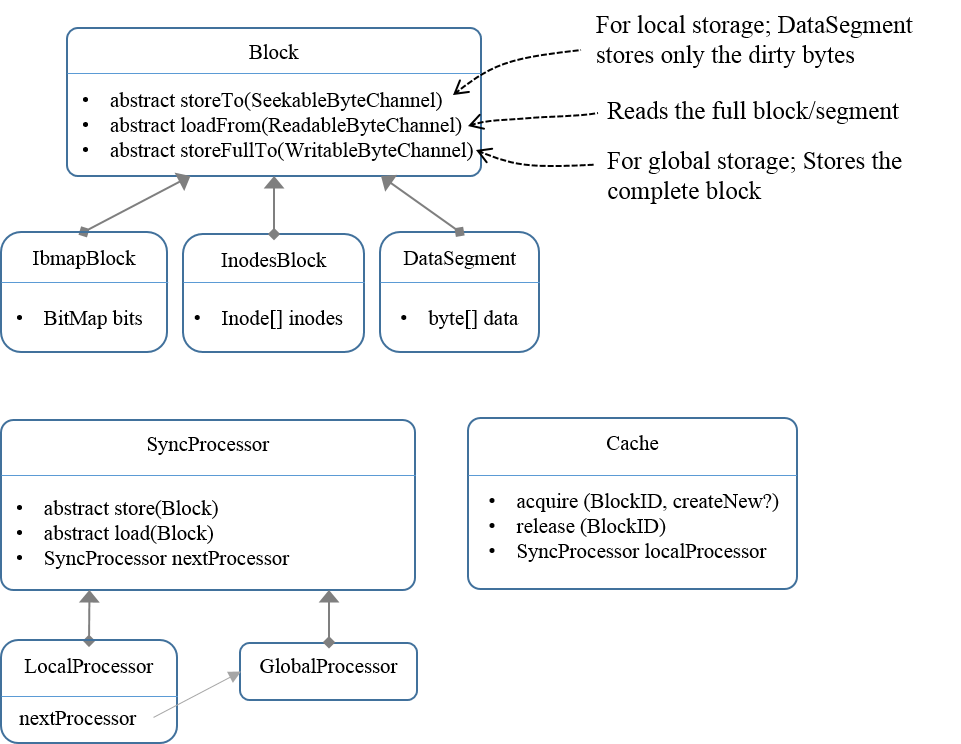
\includegraphics[width=0.9\columnwidth]{{figures/class-diagrams.png}}
%    \caption{Class diagrams.}
%   \label{fig:data-structures}
%\end{figure}



%\begin{figure}[t]
%    \centering
%    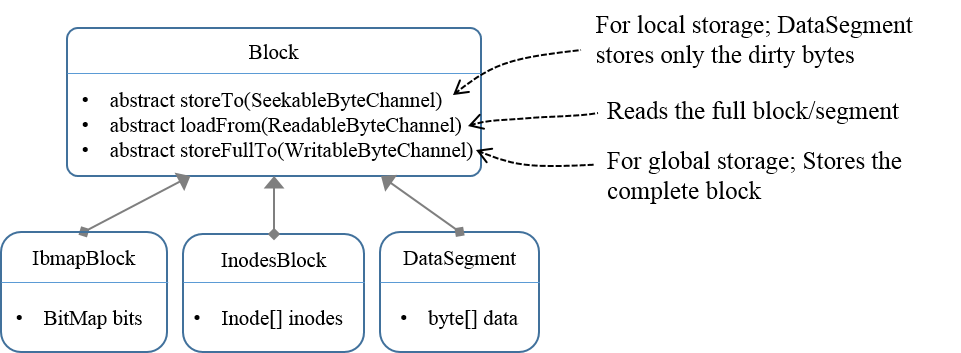
\includegraphics[width=0.8\columnwidth]{{figures/class-diagram-blocks.png}}
%    \caption{[TBD: caption] Class diagram of the blocks.}
%   \label{fig:data-structures}
%\end{figure}
%
%
%\begin{figure}[t]
%    \centering
%    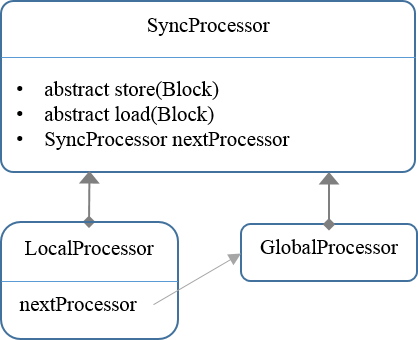
\includegraphics[width=0.4\columnwidth]{{figures/class-diagram-syncprocs.png}}
%    \caption{[TBD: caption] Class diagram of the sync-processors.}
%   \label{fig:data-structures}
%\end{figure}


%\subsection{Atomic Appends}
%
%\subsection{Reading Unfinished Block}



\section{Distributed Design of Kawkab}

This section describes the complete distributed design of Kawkab. Kawkab
supports reading incomplete blocks of data and assumes immutable global
storage. Kawkab introduces multi-version inode-blocks and data blocks to
support these features. This section details the complete distributed design of
Kawkab. However, some of the features are not implemented in the current
version of Kawkab, e.g., indirect blocks for data indexing and multi-version
blocks. The currently implemented distributed design  is described in
Section~\ref{sec:cd}.


\subsection{Distributed Metadata and Namespace}

In Kawkab, only the filesystem namespace (file directory) and other metadata
(ibmaps and inodes) are concurrently updated across the nodes. Data blocks are
not updated concurrently. Therefore, Kawkab uses a distributed key-value store
to safely and consistently store only the namespace, and it partitions the 
other metadata across the nodes.

\subtopic{Key-Value Store Consistency Requirements:} The basic requirement for
metadata consistency is that all of the nodes in Kawkab observe the same
sequence of updates to the file directory, the ibmaps, and the inode blocks.  
%As Kawkab allows only one file writer at a time, the indirect blocks, which
%contains the UUIDs of the data blocks and indirect blocks, do need to be made
%consistent across the nodes.
Therefore, the key-value store is required to provide at least sequential
consistency.
%The keys are file IDs and the values are the inode numbers in the key-value
%store.
We propose to use ZooKeeper because it allows conditional creation of the
nodes: an error is generated if a client tries to create an already existing
node. Moreover, ZooKeeper allows the clients to subscribe for notifications
when a node is updated.  These features can be used to maintain consistency
of the file directory across all the nodes in Kawkab.


\subsubsection{Data Blocks and Indirect Blocks} Data blocks are stored locally
on SSDs and remotely in the global storage such as S3. Data blocks are
not replicated to the storage of other nodes.

\subtopic{File Appends:} The file writer appends data in memory. The data
blocks are then flushed to the local SSD asynchronously for faster file write
operations. When a data block is closed, it is copied to the global storage.

\subtopic{File Reads:} Remote nodes read data blocks directly from the cache,
or from the global storage if the data blocks are not in cache.  If a
data block does not exist in the global storage, e.g., if it is the last block
in file or the block is not yet replicated in the storage, the reader
node fetches the desired block from the primary node of the file where the file
writer is located. The fetched data block is then kept in the LRU cache.

\subtopic{Indirect Blocks:} Indirect blocks, which contain the UUIDs of other
indirect blocks or data blocks, are treated the same as the data blocks.
%Indirect blocks contains UUIDs of data blocks and other indirect blocks. 
Only the file writer can update a data block or an indirect block. Therefore,
indirect blocks are stored and accessed the same was as the data blocks.


\subsubsection{Namespace Replication and Consistency}
Kawkab uses ZooKeeper to keep the namespace consistent. All the file
directory information, which consists of mappings from file IDs to the
inumbers (inode number), in ZooKeeper. ZooKeeper is a good candidate
for the namespace because the frequency of the creation of new files is low
and the higher latency for the file create operation is acceptable.

When a node creates a new file, it adds a znode in ZooKeeper on the path
\texttt{kawkab/files/fileID} and with the node-value of the inumber assigned to
the file. If the node creation fails due to an already existing znode with
the same path, it implies that another node has already created the file with the same
file ID. Therefore, the file opening for writing is failed. However, the file can be
opened for file reads in this situation. In this way, all the nodes view
the same file directory across the system.

The file directory is kept in cache on each node for faster file read and write
operations. Moreover, the file directory is periodically updated to reflect the
recent changes in the directory. This can be achieved by each node subscribing
to the znode update events for \texttt{kawkab/files}.

For the file open requests in the read-only mode, first the file directory in
the cache is used to get the inumber of the file. If the file is not found in
the cache, the node reads the file from the ZooKeeper and updates the file
directory if the file is found.



\subsubsection{Ibmap and Inodes-blocks Partitioning} Kawkab partitions the ibmap
and the inode blocks space across the nodes. Each node is assigned a specific
number of ibmap-blocks and the corresponding inode blocks.
%For example, N ibmap blocks and the corresponding inode blocks are assigned to
%each node. 
The blocks are assigned in a sequential order. The partitioning ensures that
each node uses a unique inumber for the new files without any synchronization
overhead.

\subtopic{Persistence:} Each node persistently stores its Ibmap blocks and the
inode blocks in its local storage as well as the global storage. The blocks are
periodically flushed to these storage to reduce the memory and the network usage.

\subtopic{Inode Updates Across Nodes:} Inodes are frequently updated as an inode is
updated after each file append operation to reflect the changes in the file
size and the other metadata (e.g., last modified time).  Therefore, inodes need
to be made consistent across all the readers of the file.

%\hl{Todo: How the nodes read data blocks and inodes-blocks from the other nodes.}

%Kawkab uses a simple publish-subscribe system to propagate the inodes' updates
%across the nodes where the file-readers are located. Each node with
%at least one active reader subscribes to the inode updates on the primary node
%of the file, i.e., where the file writer is located. The file writer 
%asynchronously publishes the inodes to all the subscribers. In this way,
%the staleness of the inodes is reduced on the file readers.


\subtopic{Inodes Location from Inumbers:} It may happen that a node opens a
file for reading while the file has been created by another node. As the
location of an inode cannot be inferred from an inumber, Kawkab also stores the
mapping of the inumber range to the node location in ZooKeeper.  For example,
if $x$ inodes are assigned to each node, Kawkab stores the mappings $\langle x
\to \mathrm{node1} \rangle$, $\langle 2x \to \mathrm{node2} \rangle, \ldots$,
in the ZooKeeper, which implies that the inodes from $x$ to $2x-1$ are stored
in the node with ID $\mathrm{node1}$. As this information is static and do not
change frequently, all the nodes cache this information during bootstrap. If
the information is updated due to node failures, all the nodes are updated to
reflect the changes in their cache.

\subsection{Inodes-blocks' Storage}


\begin{figure}[t]
    \centering
    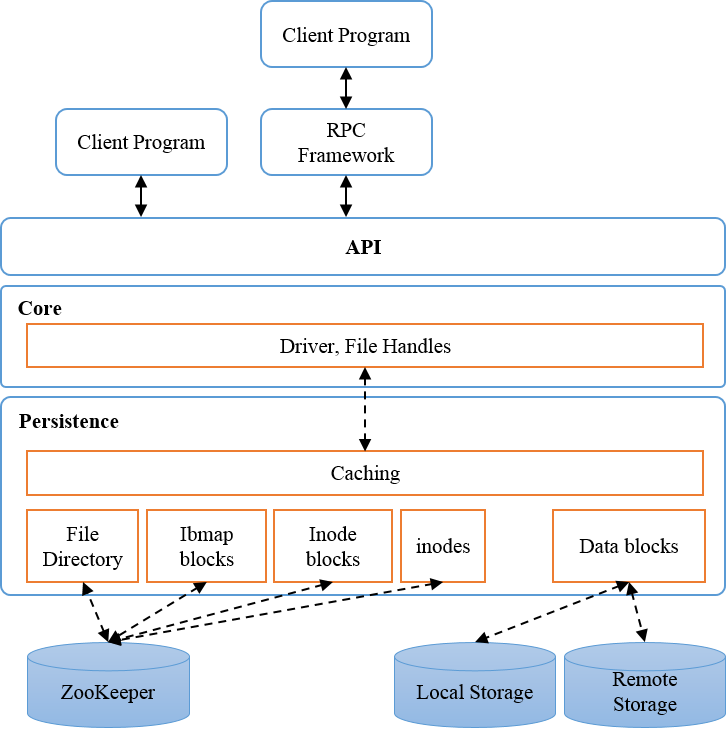
\includegraphics[width=0.83\columnwidth]{{figures/architecture.png}}
    \caption{Kawkab architecture}
   \label{fig:architecture}
\end{figure}

%
%\begin{figure}[t]
%    \centering
%    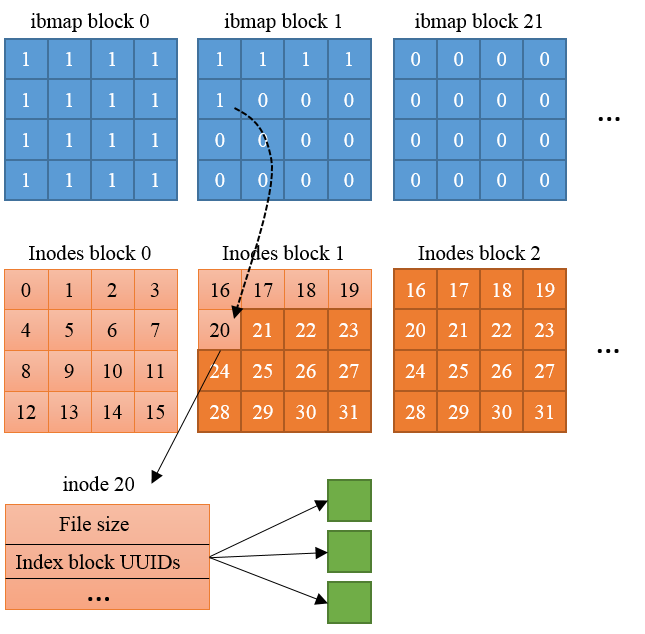
\includegraphics[width=0.5\columnwidth]{{figures/blocks-layout.png}}
%    \caption{Relationship between different types of blocks.}
%   \label{fig:blocks-layout}
%\end{figure}



%\subtopic{Problems with the Global Store:}
%
%To discuss: Why do we want to add another channel to read the inodes blocks, in
%addition to reading directly from the global store? Is it because:
%
%\begin{easylist}[itemize]
%
%# S3 is slow, which increases inodes staleness? 
%  ## What about reading inode blocks directly from the primary node, just 
%     like the data blocks?
%
%# S3 is error prone, which increases indoes staleness?
%  ## Could be solved by 
%
%# Global store or S3 could be append-only, which conflicts with the random
%  updates in inodes-blocks? This may introduce some availability problems
%  if we update the inodes-blocks using the copy-rename-delete approach.
%
%# Do we have data availability problem? For example, S3 replication is slow
%  and we want inodes-blocks to be updated immediately for all the readers.
%
%\end{easylist}

%Kawkab stores inodes blocks and data blocks persistently in a global storage
%system. Kawkab assumes that the global store is highly scalable and
%concurrently accessible to all the nodes in the system. However, the global
%system can be error prone, slow, and have append-only semantics. For example,
%Amazon S3 is a good candidate for the global store due to its high scalability and
%lower cost. However, failure rate of operations on S3 is high and S3 appends data 
%internally like an append-only system.


Inode blocks are persistently stored in the global store, which we assume to be
possibly slow, error prone, and immutable. 
%In addition, we do not impose
%any update semantics for the global storage because 
Several high performance and
scalable storage systems do not support mutable storage and atomic reads/writes~\cite{}. 
For such systems, random writes are more complex, often leading to
global locks for concurrent read and write operations. As inodes-blocks have
random update semantics, in contrast with the data blocks that are append-only,
storing inodes-blocks require different design than the data blocks
in order to avoid problems with the global store. Therefore, we introduce
multi-version inodes-blocks in Kawkab, which are further explained below.

%These can lead to several
%problems such as data staleness and unavailability for a small period.
%Moreover, some of the scalable  storage systems provide immutable object storage. 
%They might not event support atomic write operations. Random writes and
%object updates to these systems are more complex, often leading to
%retries and grabbing locks for the read/update operations.
%As inodes-blocks are also randomly written, in contrast to the append-only data blocks, 
%storing inodes-blocks in the global store is more complex. Therefore, in order
%to avoid the above mentioned problems, we introduce versioning for the
%inodes-blocks, which is further described below.


\subtopic{Multi-version Inodes-blocks:} 

%Inode blocks are persistently stored in
%a global storage system that could be slow, error prone, and might not support
%atomic updates. This could lead to data availability and staleness problems as
%the inode blocks are updated randomly in contrast to append-only data blocks.
%To avoid these problems, we introduce multi-version inode blocks. 

Kawkab stores multiple versions of inodes-blocks in the global store.  Instead
of overwriting the previous copy of an inodes-block in the global store, Kawkab
updates the version number of the block and copy the block as a new file in the
global storage. The blocks can now be located in the global store using the naming
scheme that depends on the $<$block number,  version number$>$ pairs.


\subtopic{Frequency of Creating New Versions:}

An inodes-block gets  updated on a node after every append operation for the
inodes located in the inodes-block. Therefore, the frequency of new versions
per inodes-block can be large, which can waste a lot of storage in the global
store.  To avoid this situation, we limit the frequency of creating new
versions per inodes-block by using the following policy: An inodes-block is
copied to the global storage if:
% a minimum time limit has passed since the last
%copy to the global store, and if:
%only if: % any of the following becomes true:

\begin{itemize}

\item The inodes-block is dirty and a predefined time limit exceeds after the
      inodes-block was first modified and flushed to the local storage.

\item Or, for the files corresponding to the inodes in the inodes-block, 
      the total number of new data blocks created exceed a predefined limit.
      Currently the limit is set to one data block.

\end{itemize}

This essentially coalesce several updates of the same inodes-block, which limits
the frequency of the new versions created in the global storage for a particular
inodes-block. The previous versions can be deleted after a fixed number of
version updates or a fixed time. Deletion of previous versions is simple
because inodes-blocks are simply stored as objects, blobs, or files in the
global store.


\subtopic{Keeping Track of Version Numbers:}

The versioning scheme now require recent version number propagation to the file
readers. Kawkab supports two ways to disseminate version number changes from
the primary node to the other nodes in the Kawkab cluster. First, the version
numbers are propagated through publish-subscribe channels to only the file
readers who subscribe to receive updates for specific inodes-blocks.  This
mechanism is primarily used to allow file readers to read most recent
inodes-blocks with minimal staleness. The other way to propagate inodes-blocks'
version updates is using a global distributed map. This mechanism is primarily
used when a new node joins or when the recent data is not required for file
reads. Below, first we describe the distributed map and then we discuss the
pub-sub approach for version changes propagation.

\subsubsection{Inodes-block-versions Table}

Adding version numbers for the inode blocks require keeping track of the
current version number for each inodes block. Therefore, we introduce a global
distributed table called \textit{inodes-block-versions table} (IBV table),
which  stores the recent version number for each inodes block. Any distributed
key value store, e.g., ZooKeeper and DynamoDB, can be used as the IBV table. 

In the IBV table, we store the version numbers of all the inodes-blocks
assigned to the nodes in Kawkab. The IBV table maps Kawkab node IDs to a list
of $<$inodes-block number, recent version$>$ tuples for all the inodes-blocks
created by the node. The list is expected to be small, at most a few kilobytes, 
because the list
contains the block and version numbers for only the block that the node
has created.  The number of inodes-blocks created per node is not huge, 
even though the total number of files created can be very large,
because each inodes-block consists of a large number of inodes. 

\subtopic{Consistency Requirements:}

The IBV table is required to be at least eventually consistent.  Eventual
consistency is sufficient for the IBV Table because Kawkab allows only one file
writer per file at a time.
%ventually consistent IBV table does not introduce the problem of data onflicts
%in Kawkab because  Kawkab allows only one writer per file at a time.
Therefore, the updates to the same data in the IBV table originate from only
one source, which cannot create data conflicts.

\subtopic{IBV-table Update Frequency:}

A possible problem with the IBV table could be that the high request rate to
the IBV table may limit the scalability of the system. Inodes-blocks are
frequently updated as each append operation updates an inode. This could lead
to a high rate of version number updates that can overwhelm the IBV table.
However, this situation is unlikely because we already throttle the frequency
of new versions created in the global store for each inodes-block.  In
addition, we limit the updates to the IBV table by adding a minimum time bound
between the subsequent updates. The minimum time
could a large value such as tens of seconds because the IBV table is 
supposed to be mainly used when a new node joins the Kawkab cluster or when a node
reads non-recent data from the file.


\subsubsection{Versions Propagation Using Pub-sub Channels}

Limiting the frequency of updates to the inodes-blocks adds staleness in the
data stored in the IBV table. Therefore, we add a pub-sub system in Kawkab that
allows readers to receive the most recent version changes for specific
inodes-blocks. The readers subscribe to the writers for particular
inodes-blocks to receive version change updates. The writers publish the recent
version number of an inodes-block after copying the inodes-block to the global
store. In this way, the readers can read the most recent inodes-blocks
available in the global store.
%\footnote{Another option could be to publish inodes to the subscribed readers,
%instead of just publishing the version numbers of the blocks. This will allow
%the readers to read most recent data with minimal staleness.} 
For implementation, we can either use ZooKeeper for this purpose, which may
become the bottleneck, or use a specialized system such as Apache Kafka and
Chronicle Queues.


\subsubsection{Reading Unfinished Blocks}

Unlike other system~\cite{}, Kawkab allows the readers to read unfinished data
blocks. The readers can either read unfinished blocks from the global store, or
from the primary nodes of the files. Reading from the primary node is a simple
RPC request. However, storing partially filled blocks in the global store
require random updates and mutability in the global store, which is not always
possible. Therefore, like the inodes-blocks, Kawkab adds multi-version support
for only the last data block of the virtual files.

\subtopic{Storing Partially Filled Data Blocks:}
A node copies the dirty and partially filled data blocks in the global store after
a predefined time limit, e.g., after two seconds since the last append operation.
The data blocks are assigned the next version number when the data blocks are copied 
in the storage. 

\subtopic{Current Version of the Last Data Block:} The current version number
information of the last data block of a file is stored in the inode associated
with the file. The version number is updated in the inode after copying the
last data block in the global storage with the new version number.

\subtopic{Version Number of the Complete Data Blocks:} 
The complete data blocks for a file are assigned a default version number, e.g.,
version zero.

\subtopic{Locating the Last Data Block:} The last data block can be located
based on the \texttt{inumber-blockNumber-versionNumber} combination.

\subtopic{Garbage Collection of Data Blocks:}
The obsolete partially filled data blocks can be deleted after some predefined
time. The time should be greater than the inodes-blocks version update time.
This is because a reader may read stale inode and try to read the older version
of the block even though the newer version is available in the global store.


\subtopic{Propagating Last-block's Current Version:}
The current version of a file's last block is stored in the inode of the file.
Therefore, the readers require the most recent inode in order to read the
latest version of the data block. Kawkab provides pub-sub channels to propagate
the most updated inodes to the subscribed readers.

In this approach, the readers, which we expect to be small in number, subscribe
to the primary nodes to receive the most updated inodes for the particular
files. The primary nodes broadcast the inode whenever the inode is updated. An
inode is updated after each append operation and when the version number of the
last data block is updated.

The benefit of this approach is that the partially filled data blocks
can be read from the global store instead of the primary nodes. This reduces
load from the primary nodes and provides better scalability with the number
of readers in the system.



\section{Current Distributed Design}
\label{sec:cd}

\begin{figure}[t]
    \centering
    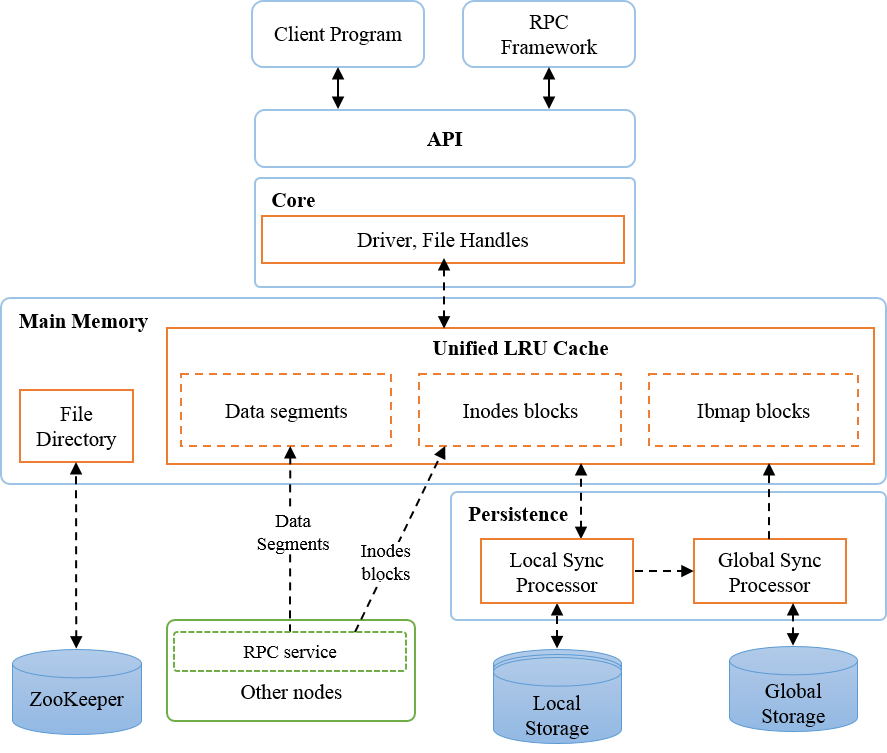
\includegraphics[width=0.7\columnwidth]{{figures/current-design.png}}
    \caption{Design of Kawkab in the current implementation}
   \label{fig:current-design}
\end{figure}




Kawkab filesystem design is built around three types of blocks: ibmaps,
inodes-blocks, and data blocks. These blocks have different access patterns and
update semantics: Ibmaps and inodes-blocks are mutable and have random writes,
whereas data blocks are immutable and allows only append operations. 

An ibmap is updated after each file creation or deletion, and an inodes-block
is updated after each append operation on a file whose inode is in the
inodes-block.  However, our original assumption that the global store does not
support object modifications and rewrites restricts the storage of ibmaps and
inodes-blocks. The proper solution is to store the mutable blocks in multiple
versions and maintain versioning information. However, the current
implementation lacks multi-version inodes-blocks and data blocks functionality.
Therefore, in the current implementation, we relax our assumption about the
global store and assume that the store supports object rewrites, which allows
us to update and rewrite inodes-blocks in the global store.
Figure~\ref{fig:current-design} shows the architecture of Kawkab in the
current implementation.

%Following is the detail of the design we have followed in
%the current implementation to work without multi-version blocks.


\subtopic{Persistence in the Local Store:} All the blocks are placed in a
\textit{LocalStoreQueue} after modifications in the blocks. A predefined number
of worker threads take blocks from the queue and rewrite them in the local
store.  As the workers can be slower than the readers and writers that add
blocks in the queue. Therefore, to prevent the queue from growing fast and
indefinitely, a block is added in the queue only if the block is not already in
the queue. This also coalesce several updates in memory in a single
synchronization to the local store.  Each block has an associated
\textit{localDirtyCount} that allows the workers to check if the block was modified
while flushing to the local store. If the block is still dirty after flushing
to the local store, the block is added again in the queue. 

%LocalStoreQueueu is maintained such that the queue's size does not grow fast if
%the update rate of the same blocks is faster than their the rate of 
%their synchronization with the local storage. 
%An inodes-block update rate can be very high due to the large number
%of inodes per block. This may create a situation in which a 
%a block that is already in the LocalStoreQueue is 
%updated again and added again in the queue before  a worker thread
%removes the block from the queue and flush to the local store. 
%In this way, the queue size will keep increasing that will
%use a large memory portion. To prevent this situation, a block is added
%in the LocalStoreQueue only if the block is not already in the queue.



\subtopic{Persistence in the Global Store:} Following the same approach to
store the blocks in the local storage, the dirty blocks are placed in the
\textit{globalStoreQueue} to be transferred in the global store. Predefined
number of workers take blocks from the queue and store them in the
global storage. Each block has an associated \textit{globalDirtyCount}
to support coalescing multiple updates and to identify if the block
is required to be stored or rewritten in the global store or not.
Although the storage mechanism is similar, the global storage is different 
than the local storage in the following two aspects.

First, ibmaps and inodes-blocks have a different storage policy as compared to
data blocks. Ibmaps and inodes-blocks are rewritten in the global store as fast
as possible. However, the updates are coalesced because a block is not added in
the queue if it is already in the queue or being stored in the global store. If
the block still remains dirty after storing to the global store, the block is
added again in queue. In comparison, data blocks are added in the global store
only when the blocks become full with file data.  Moreover, data blocks are
never updated or rewritten in the global store.  This implies that the
incomplete blocks are not available in the global store for the readers.
Therefore, the readers fetch the incomplete blocks from the primary nodes,
which we further discuss later in this section.

Second, the storage to the global store is slower than the storage to the local
store. As a result, it may happen that some data block segments may not be in
the cache when the block is prepared to be copied to the global storage.
Therefore, a block is copied to the global store by reading from the local
store instead of the cache. Thus, the local store workers sync blocks from the
cache to the local store, and the global store workers sync blocks from the
local store to the global store by reading files from the underlying
filesystem. This mechanism allows the cache to evict blocks that are synced to
the local store but are still pending to be copied to the global store.  In
this way, Kawkab can keep up with fast data ingestion rates while taking
benefit of a hierarchy of storage levels with different read and write
throughputs. 

\textit{A nuance in the implementation:} Practically, the current
implementation has a different model than described above because of the lack
of multi-version blocks functionality. In the current implementation, Kawkab
uses S3 API to copy blocks to the global store by reading files from the local
storage. For fault-tolerance, S3 API calculates an MD5 hash of the file before
transferring the block to the global store. If the file hash changes before
completing the storage to the global store, S3 API throws an exception
complaining that the block's hash has been modified. Therefore, a block cannot
be synchronized from the cache to the local store while the block is being
transferred to the global store. This results in longer local storage latency
-- a block's local storage completes only when the block has been updated in
the global store. This allows Kawkab to coalesce many block updates in a single
local and global storage task. The drawback of this approach is the blocks take
longer time the cache and the cache efficiency is lower than its potential.
However, this functionality will be improved when the multi-version blocks
support will be added in the system.

\subtopic{Cache Eviction Policy:}
A reader or a writer acquires a block from the cache for reading or writing,
and then release the block to the cache after completing its task\footnote{A
block can be acquired concurrently by a single writer and multiple readers}. 
The cache keeps track of the block's references using a reference counter. The
cache increments the reference counter when the block is acquired and it
decrements the counter when the block is released. In addition, the cache adds
the block in the localStoreQueue if the block is dirty when the block is
released.

When a block is acquired, the cache brings the block in the cache if it is not
already in the cache. If the cache runs out of capacity, the cache evicts the
least recently used (LRU) block from the cache.  A block can only be evicted
from the cache if its reference count is zero. If the LRU block's reference
count is greater than zero, the cache searches the next item in the LRU
queue, until it finds a zero-referenced block and evicts that block from the
cache.

\textit{Back-Pressure:}
During peak data ingestion rates, it may happen that the LRU block with
zero reference count has dirty bits because the block may still be in the
localStoreQueue. If the LRU block that is being evicted has dirty bits,
the cache blocks until the block is synchronized with the local store.
This provides automatic back pressure, preventing the system to be
overloaded.


\subtopic{Local Store Eviction Policy:} Local store's eviction policy is
different for different blocks. As ibmaps use a small amount of local storage
space, ibmaps are never evicted from the local store. Inodes-blocks also use a
small storage space, however, inodes-blocks are frequently updated. Therefore,
inodes-blocks are also not evicted from the local store. Major portion of the
local store consists of data blocks.  A data block from the local store can
only be evicted if the block is not the cache and the block is fully
synchronized in the local and the global store.  When the cache evicts a block,
the cache notifies the local store that the block is being evicted. The local
store then evicts the block if the block's policy allows it, i.e., if the
evicted block is the last segment of a data block.  A data block can be evicted
from the local store even if some of its segments are in the cache as those
segments are read-only: The block is synchronized to the local and the global
store before eviction, which is described earlier in this section.
Evicted blocks from the local store are deleted from the underlying filesystem
of the local storage. 

Local store keeps track of the blocks available in the local store through a
persistent key-value store. The current implementation uses Chronicle Map
library to persistently store the information about the blocks that are stored
locally.


\subtopic{Reading Blocks from Primary Nodes:} Readers on non-primary nodes
fetch blocks from the global store.  However, the global store does not store
incomplete blocks and the stored inodes-blocks may be staled. Therefore, the
readers on the non-primary nodes read last incomplete blocks and fresh
inodes-blocks from the blocks' primary nodes using an RPC service.  

Each node provides an RPC interface that allows the readers on non-primary
nodes to read inodes-blocks and data blocks that are owned by that node.  A
read follows the following procedure to read block that is not already in the
cache. A Reader on a non-primary node first tries to read the block from the
global store.  If the block does not exist in the global store, the reader
requests the block from the block's primary node using an RPC sevice. The
primary node reads the block from the local store and sends back to the reader.
However, it may happen that the primary node have deleted the block before
received the request. In this case, the primary node returns BlockDoesNotExist
error to the reader. The reader then retries to fetch the block from the global
store. If still the block is not found in the global store, this implies an
implementation error as the block must be in either local store, global store,
or the both.


\textit{Data Expiry Time:} A node expires an incomplete last block and inode-blocks
fetched from the primary node after a predefined time period. 
This is because the cache only evicts a block when it runs out of space. However,
the inodes-blocks are updated frequently. In order to fetch recent inodes-blocks
and last data blocks, the blocks are expired but not evicted from the cache.
An expired block requires reloading from the global or the primary node when
the block is acquired from the cache. In this way, the nodes read most of the
data blocks from the global store, and the incomplete blocks and inodes-blocks
from the primary node.



%\section{Implementation Details}
%
%- Thread model
%- Cache model
%  - How to acquire and release blocks from the cache
%  - Cache eviction policy
%- Local store manager
%- Global store manager
%- Synchronization between the cache, the local store and the global store managers






%\section{Related Work}
%
%\begin{easylist}[itemize]
%
% # Comparison with Alluxio
%
% # Comparison with Succinct
%
% # Comparison with HDFS and similar systems
%
%\end{easylist}
%






%- The objective is to allow the readers to read the unfinished blocks
%  from the global store. Moreover, it reduces data loss for the last blocks
%  in the case of node failures.
%
%- We add versioning for last data block
%
%- Inode keeps track of the version number of the last data block
%
%- A complete block gets a default version number, e.g., version zero.
%
%- The unfinished dirty data blocks are periodically copied to the global store 
%  by updating version numbers.
%
%- The version number change for the last block is also added in the inode.
%
%- The inode change is published to the subscribers periodically.
%

%- TODO: Node failures. Now we have multiple levels when a failure can happen.

%- To discuss: When to delete the older version data blocks? What if a reader tries to read a 
%  partially filled data block from the global store, but the block has been deleted because
%  the block is completed and moved to the default version number? The reader either require
%  the most updated inode, or it need to retry using the default version number of the
%  block.


%\subsubsection{Inodes Propagation Using Pub-sub Channels:}
%
%
%- We publish individual inodes as well through the pub-sub channel. The objective
%  is to reduce staleness for the inodes and to allow readers to read the unfinished blocks.
%
%
%- Inodes are only published to the subscribers, which are expected to be small
%  in number.
%
%- Inodes will be published periodically, with a small time bound in milliseconds, e.g.,
%  100ms.
%
%
%
%- TODO: Does a node subscribes to all other nodes?
%
%- TODO: Should a node publish the map of inodes-blocks and their versions
%  instead of the versions of individual inodes-blocks?


%\subtopic{Performance Implications:}
%
%Pub-sub shares the upload bandwidth with the data transfers to the global
%store. Moreover, an inode read may follow a data block read. Therefore, enough
%large number of publications in the pub-sub channels may slow down data
%transfer to the global store, which may lead to overflow in the local storage.


%\subtopic{Alternate Design: Storing Inodes in DynamoDB:} TBD
%Another way to store inodes is to place the inodes in a key-value store such as
%DynamoDB. Howe


%\subtopic{Alternate Design: Storing Inodes-blocks in DynamoDB:} TBD

%\subtopic{Other Options: Recent Data blocks:}
%
%- If a reader reads the most recent inode, it may also want to read the last
%data block, which will most likely be not available in the global store yet.
%Therefore, the most recent inode read likely follows the last or a few recent
%blocks. This implies that the inode reads and the recent data block reads have
%high correlation. Therefore, we may want to add pub-sub for data records
%instead inodes-block versions.

%\subtopic{To be discussed:}
%
%- A drawback of the block location based on inumber is that if any operation
%  involves changing the inumber, then the operation will be very expensive: it
%  will require copying everything using the new inumber and then deleting the
%  previous one.


\begin{algorithm}[ht]
\label{alg:journal}
\caption{Write-ahead log's journal entries to tolerate failures during append operations}
\begin{algorithmic}[1]
\item[]
\Struct{\textbf{For an append operation}} 
\State Data to append
\State New file size
\State Append data block
\State Update inodes-block: Update file size in the inode
\EndStruct
\item[]

\Struct{\textbf{For creating a new data block without creating a new data block}}
\State Data to append
\State New file size
\State Create data block locally
\State Append data in the first segment
\State Schedule to copy recently completed block block to the global store
\State Schedule to copy inodes block to the global store
\State Update inode: File size and last block version
\State Update IBV-table with the new inodes-block version
\State Send updates to pub-sub channels if there are any subscribers.
\EndStruct
\end{algorithmic}
\end{algorithm}


\section{Future Work}

The current design of Kawkab allows to read files using file offset only.
Moreover, the current design does not include the proper failure handling 
model of file operations. Below we give high level overview of these two 
features that will be added in Kawkab in the future.


\subsection{Extensible Indexing}

Currently Kawkab allows the readers to read files from a specific
byte number in the file. Extensible indexing will allow accessing structured
data through at a given index such as timestamp. Moreover, extensible indexing
will support pluggable indexing for different types of files.

%Kawkab is an append-only system. Each append is performed at the end of the file.
%However, a file can be read from any location. When a client opens a file,
%it is returned a FileHandle. The FileHandle contains a read pointer that indicates
%the current position in the file from where the data will be read. The read
%pointer can be moved to any position in the file using any of the following
%ways: 
%
%\begin{enumerate}
%  \item Move to an absolute byte offset in the file.
%  \item Given a timestamp T:
%  \begin{itemize}
%    \item Move to the first byte of the closest block that has the append time equal to
%          or \textit{before} T
%    \item Move to the first byte of the closest block that has the append time equal to
%          or \textit{after} T
%  \end{itemize}
%\end{enumerate}
%
%In order to find the data block that contains the given byte or timestamp, Kawkab
%performs binary search over the index in the inode.
%
%\begin{itemize}
%  \item Indexing within a block
%  \item Time range queries
%\end{itemize}
%
%%  - How data is indexed
%% - How data is retrieved given a byte offset
% % - How data is retrieved given a timestamp
%
\subsection{Fault Tolerance}

Several operations in Kawkab consist of multiple stages while the operations need 
to be atomic. For example, an append operation consist of updating data in-memory and
the local store, and potentially creating a new block in the global store. If such
operations fail at any stage, the whole operation need to be cancelled. In order
to handle failures without corrupting the file system, we implement journaling
at the local level at each node. In the current version, we implement both
data as well as metadata journaling that will ensure that the system is always
in a recoverable and consistent state. We expect that journaling will have low
performance overhead because journaling is performed locally per node and the
journal is appended asynchronously on the local disk. However, if we find significant
performance overhead due to data journaling, we will implement only metadata journaling
in the file system.

\subsection{Append Operation}

Table~\ref{alg:journal} shows (i) the journal entry for an append operation that does not cause creation
of a new inodes-block version and new data block, and (ii) the journal entry for an append
operation that creates a new data block.




\section{Summary}
Kawkab is a distributed filesystem that is designed to handle large volumes
of streaming data that is common in financial industry. Kawkab can efficiently
handle fast incoming data by utilizing a hierarchy of storage mediums:
main memory, local storage such as SSDs, and a global storage such as Amazon S3.
These storage mediums provides a hierarchy of read and write latencies.
Kawkab uses the hierarchy to handle bursts of high data ingestion rate.
In this document, we have detailed the distributed design of Kawkab.

The current implementation of Kawkab runs on multiple nodes, accesses
a global storage through an S3 client library, allows reading data from
primary nodes, and supports reading and writing data in binary format.
The current version does not support reading incomplete blocks from the
global storage, which may restrict a node from opening a large number
of files on the same node.
The next version of Kawkab will include multi-version blocks that
will allow the nodes to move incomplete blocks to the global store. Moreover,
the next version will include the mechanism to read blocks with lower
staleness. In the future, Kawkab will include structured files, extensible
indexing, and operation level journaling for high fault tolerance.




%\subsection{Scalability}
%
%\begin{easylist}[itemize]
%
%  # Scaling with the number of nodes
%    ## Can scale with the number of nodes because:
%      ### Nodes do not interact with each other for the read and append operations
%      ### Global storage is assumed to be scalable
%
%    ## Bottlenecks can be:
%      ### Reading most recent data
%      ### Frequent access to the file directory
%%
%  # Scaling requests per node
%    ## Bottlenecks:
%      ### Limited RAM and LRU cache
%      ### Local storage
%        #### Can be reduced by using multiple SSDs or EBS
%      ### Global storage
%      ### Locks around the cache
%
%\end{easylist}
%


%\subsection{Fault-tolerance}
%
%\begin{easylist}[itemize]
%
%# File append operations
%  ## Before writing to the local storage, appends are not fault-tolerant
%  ## Data blocks are copied to the global storage only after the blocks are full. We may need to copy
%     them to the global storage
%
%# Node failures
%
%# What if the global storage is not available?
%  ## Global store failures: assume that the global store will not fail due to enough data replication
%
%# Failed get and put operations
%
%
%\end{easylist}
%
%\subsection{Consistency Guarantees}
%
%- Strong consistency, single writer
%
%- Data loss due to power or machine failures
%
%%We guarantee strong consistency, however, the data may be lost if the node fails before coping the
%%data to the global store. Isn't it a weak strong consistency ;)
%
%\subsection{Metadata and Data Journaling}
%
%We need metadata and data journaling to ensure atomic operations and recovery from failures. However,
%this will slow down the filesystem's performance. 
%
%
%
%%\subtopic{Creating a New File:}
%%\begin{itemize}
%%  \item Get inumber \texttt{inum} from the ibmap
%%  \item Execute a multi-operation transaction in ZooKeeper:
%%  \begin{itemize}
%%    \item Create a persistent node with path \texttt{kawkab/inodes/inum}.
%%    \item Create a persistent node with path \texttt{kawkab/files/fileID} and the value equals to \texttt{inum}.
%%  \end{itemize}
%%  \item If the previous transaction succeeds, update the local file directory and the ibmap.
%%  \item If the transaction fails, it is because either (1) The inode is already consumed, or (2) the file already
%%        exists. If the file already exists, then the file creation operation returns with FileExists error. If the
%%        inode is already consumed, 
%%\end{itemize}
%
%
%%\subsection{Distributed Namespace:}
%%Kawkab partitions the namespace across all the nodes. Each node has a dedicated
%%namespace, and each node creates new files in its own namespace. The metadata
%%belonging to each namespace -- files directory, ibmaps, and inode blocks --
%%are kept consistent across all the nodes.
%
%%\section{File Read and Write Operations}
%
%
%
%
%%\subsection{File Create Operation}
%%
%%Following is the journal entry when a new file is created:
%%
%%\begin{itemize}
%%\end{itemize}
%

\end{document}

